\section{Datum}
\subsection{Pengertian DATUM}

Datum reference surface atau geodetik atau georeferensi adalah parameter sebagai referensi untuk mendefinisikan geometri Bumi ellipsoid. Datum geodetik diukur menggunakan metode manual agar lebih akurat lagi menggunakan satelit.

Dibawah ini merupakan Jenis geodetik menurut metodenya :
\begin{enumerate}
\item Datum horizontal adalah datum yang digunakan untuk pemetaan horisontal. Dengan teknologi yang lebih maju, kini muncul tren penggunaan datum horizontal dari koordinat geosentris global sebagai penggganti datum lokal atau regional.
\begin{figure}[htbp]
		\centering
		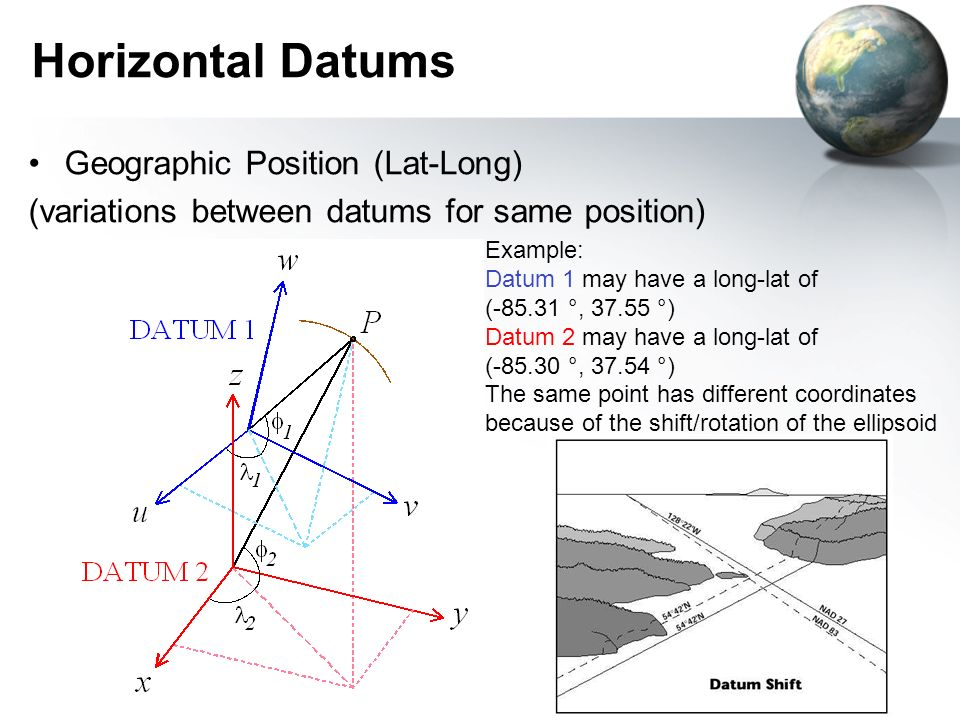
\includegraphics[width=0.75\textwidth]{pictures/datum_horizontal.jpg}
		\caption{Datum Horizontal (Sumber : https://www.slideshare.net/AeroMetri)}
		\label{Datum Horizontal}
		\end{figure}	

\item Datum vertikal adalah sistem referensi untuk ortometris medan tinggi. Datum vertikal digunakan untuk mewakili ketinggian atau kedalaman informasi. Biasanya bidang referensi yang digunakan untuk ortometris sistem tinggi adalah geoid.
\begin{figure}[htbp]
		\centering
		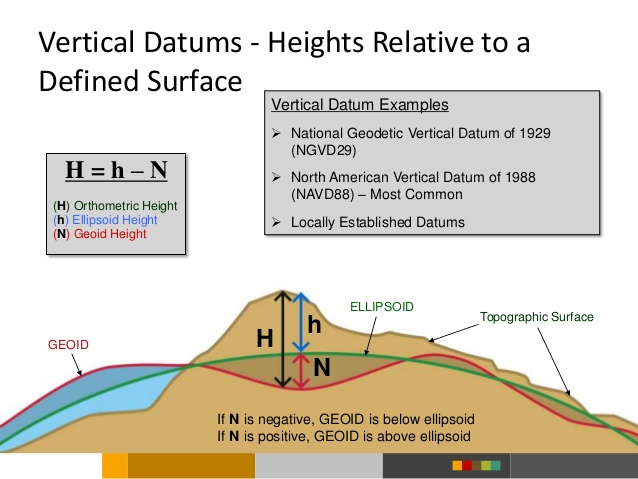
\includegraphics[width=0.75\textwidth]{pictures/vertical_datum.jpg}
		\caption{Datum Vertikal (Sumber : Map Projections and Coordinate Systems 2014)}
		\label{Datum Vertikal}
		\end{figure}	
\end{enumerate}

Sedangkan menurut jenisnya datum geodetik menurut luas areanya :
\begin{enumerate}
\item Datum geodetik lokal adalah bentuk geoid yang paling cocok pada area yang tidak terlalu besar. Sampel datum lokal di Indonesia antara lain: Genoek, datum Monconglowe datum, di 74 (Datum Indonesia 1974), dan dengan 95 (Datum Geodetik Indonesia 1995).
\begin{figure}[htbp]
		\centering
		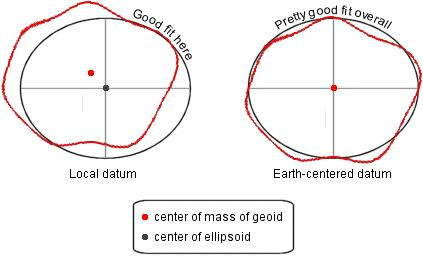
\includegraphics[width=0.75\textwidth]{pictures/datum_geotik_lokal.jpg}
		\caption{Datum geodetik lokal (Sumber : Map Projections and Coordinate Systems 2014)}
		\label{Datum geodetik loka}
		\end{figure}	

\item Datum referensi geodetik regional ellipsoid adalah dengan menggunakan bentuk yang paling sesuai dengan bentuk permukaan geoid ke area yang relatif lebih luas dari datum lokal. Datum regional biasanya dibagi oleh Negara yang berdekatan dengan negara yang terletak di satu benua. Contohnya termasuk: datum datum regional dan datum NAD Indian (North-American Datum) 1983 yang merupakan datum untuk negara-negara yang terletak di bagian utara Amerika, Eurepean 1989 Datum digunakan oleh negara negara yang terletak di benua Eropa, dan Australia Datum Geodetik digunakan pada tahun 1998 yang terletak di benua Australia.
\begin{figure}[htbp]
		\centering
		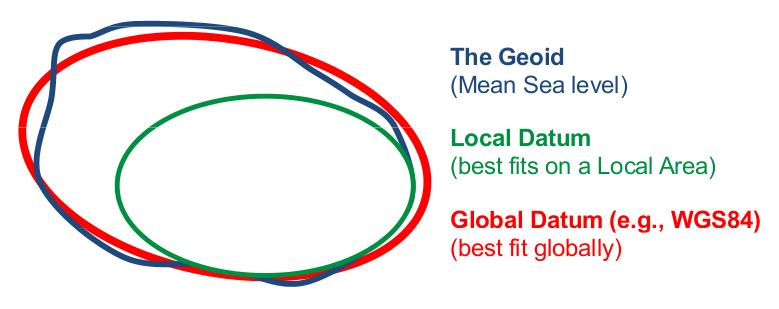
\includegraphics[width=0.75\textwidth]{pictures/datum_referensi_geodetik_regional_ellipsoid.jpg}
		\caption{Datum referensi geodetik regional ellipsoid (Sumber : Nauipedia)}
		\label{Datum referensi geodetik regional ellipsoid}
		\end{figure}	

\item Global Datum datum geodetik adalah referensi ellipsoid untuk digunakan sesuai dengan bentuk geoid dari seluruh permukaaan Bumi. Karena penggunaan datum yang berbeda di negara yang berdekatan serta karena perkembangan teknologi positioning yang sedang mengalami kemajuan pesat, maka penggunaan datum menunjuk ke datum global. Datum datum global pertama adalah WGS 60, WGS66, WGS 72, pada awal tahun 1984 mulai digunakannya datum WGS 84, ITRF dan (Sistem Referensi Terestrial Internasional).
\end{enumerate}

\subsection{Pengertian WGS 84}
World Geodetic System adalah standar untuk digunakan dalam kartografi, geodesi, dan navigasi. Terdiri dari kerangka koordinat standar untuk Bumi, permukaan referensi standar bulat (datum atau referensi ellipsoid) untuk data ketinggian mentah, dan gravitasi permukaan ekuipotensial (geoid) yang mendefinisikan permukaan laut nominal. 
Revisi terakhir adalah WGS 84 (berasal dari tahun 1984 dan terakhir direvisi pada 2004), yang berlaku hingga sekitar 2010. Skema sebelumnya termasuk WGS 72, WGS 66, dan WGS 60. Sistem referensi koordinat WGS 84 digunakan oleh Sistem Pemosisian Global.

\subsection{WGS 84 Sebagai Penentuan Posisi}
Datum digunakan untuk penentuan posisi GPS yang disebut WGS84 (World Geodetic System 1984). Ini terdiri dari sistem koordinat kartesius tiga dimensi dan ellipsoid saling terhubung, sehingga posisinya dapat digambarkan sebagai koordinat WGS84 XYZ Kartesius atau lintang, bujur dan koordinat elipsoid. Asal datum adalah Geocentre (pusat massa Bumi) dan dirancang untuk memposisikan mana saja di Bumi.
 
Sejalan dengan definisi datum, datum WGS84 yang disediakan, tidak lebih dari satu set konvensi, mengadopsi formula dan konstanta. Tidak ada infrastruktur fisik yang disertakan, dan definisi tersebut tidak menunjukkan bagaimana Anda dapat memposisikan diri dalam sistem ini. 

Posisi satelit WGS84 ditentukan oleh Departemen Pertahanan AS menggunakan jaringan stasiun pelacak, posisi yang telah dihitung secara tepat. Stasiun pelacakan mengamati koordinat satelit dan WGS84, yang menentukan, dari satelit. Kualitas koordinat satelit kami dihasilkan tergantung pada kualitas koordinat pelacakan stasiun yang diketahui. awalnya tidak terlalu bagus (mungkin akurasi sepuluh meter) tetapi telah disempurnakan beberapa kali. Kumpulan koordinat terbaru, termasuk pelacakan tiga belas stasiun yang didistribusikan di seluruh dunia, diperkenalkan pada Januari 2002. Sekarang pelacakan stasiun koordinat akurat hingga lebih dari lima sentimeter, dan dalam perjanjian yang sangat dekat dengan International Reference Meridian dan International Reference Reference .

Jaringan stasiun pelacakan GPS dapat dianggap sebagai WGS84 TRF asli. Konstelasi satelit, yang merupakan turunan TRF, dapat dilihat sebagai alat untuk mentransfer realisasi ini ke cakrawala ke mana pun posisi yang diperlukan di dunia. Koordinat saat ini dari stasiun pelacakan antena Apennine 1997.0 tersedia di Internet (lihat bagian 8 untuk alamat). Koordinat tersirat ini menyatakan asal, orientasi, dan skala sistem fisik: mereka telah dihitung sedemikian rupa sehingga elemen-elemen ini sedekat mungkin dengan persyaratan teoritis yang tercantum dalam bagian 4.1. Tentu saja, tidak ada TRF yang sempurna, ini mungkin bagus untuk lima sentimeter atau lebih.

Sebelum Mei 2000, keakuratan stasiun pelacakan A.S. yang penuh dengan TRF tidak tersedia bagi pengguna non-militer. Dalam pemindahan posisi satelit ke TRF ini, posisi akurasi sengaja digabungkan dengan fitur yang dikenal sebagai ketersediaan selektif (SA). Ini berarti bahwa pengguna sipil dengan satu penerima GPS tidak dapat menentukan posisi WGS84 dengan akurasi lebih baik sekitar 100 meter. Pada bulan Mei 2000, degradasi yang disengaja dari sinyal GPS ini secara resmi dimatikan.

Dengan sepasang penerima GPS, kami dapat mengukur posisi relatifnya secara akurat (mis., Vektor tiga dimensi antara dua penerima dapat ditentukan secara akurat). Kita harus meletakkan salah satu penerima pada titik yang terkenal dan meninggalkannya di sana. Ini dikenal sebagai GPS posisi relatif atau GPS diferensial. Untungnya, ada metode untuk secara akurat menentukan posisi WGS84 nyata dari yang diketahui dan, oleh karena itu, mengembalikan posisi WGS84 yang benar.

\subsection{Pengertian NAD 83}
NAD83 adalah akronim untuk Amerika Utara tahun 1983, datum geosentris dan sistem koordinat geografis berdasarkan Geodetic Reference System 1980 (GRS80) ellipsoid. Ini terutama digunakan di Amerika Utara, data pengukuran diperoleh dari satelit dan terestrial. NAD83 mengoreksi beberapa distorsi yang melekat dalam survei jaringan NAD27 yang telah terakumulasi dari waktu ke waktu dan jarak. NAD83 juga memiliki kelebihan sebagai datum asli yang digunakan oleh teknologi survei satelit modern seperti Global Positioning System (GPS).

Realisasi NAD83 pertama kali diperkenalkan pada tahun 1986 oleh sekelompok lembaga yang mewakili berbagai negara di Amerika Utara untuk meningkatkan sistem referensi sebelumnya; itu adalah Datum Amerika Utara 1927 tahun atau NAD27. Secara khusus, Survei Geodesi Nasional (NGS) mewakili Amerika Serikat, dan Pemerintah federal secara resmi merujuk pada realisasi NAD83 pertama sebagai NAD83 (1986). Untuk merealisasikan hal ini, kelompok-kelompok lembaga sangat bergantung pada pengamatan Satelit Doppler yang dikumpulkan di beberapa ratus situs untuk memperkirakan lokasi pusat massa Bumi dan orientasi sumbu 3D Cartesian.

Sistem referensi spasial NAD83 digunakan untuk georeferensi nasional oleh sebagian besar lembaga federal dan provinsi di Kanada. Realisasi fisik dari sistem ini telah mengalami beberapa pembaruan sejak pertama kali diperkenalkan pada tahun 1986. Telah berevolusi dari jaringan kontrol horizontal tradisional realisasi 3D berbasis darat menjadi teknik berbasis ruang yang sepenuhnya mendukung pemosisian yang lebih modern dan integrasi kedua sistem secara horizontal. dan sistem referensi vertikal. Setelah tinjauan singkat dari sistem referensi sebelumnya yang digunakan di Kanada, definisi asli NAD83 dan pembaruan berikutnya dijelaskan, dengan fokus pada implementasi definisi NAD83 saat ini (sistem referensi spasial Kanada, CSRS) dan hubungannya dengan sistem referensi lainnya. Parameter transformasi resmi antara NAD83 (CSRS) dan Frame Referensi Terestrial Internasional (termasuk WGS84) disediakan untuk digunakan di seluruh Kanada. Kemungkinan sistem referensi di masa depan untuk Kanada dan Amerika Utara juga diperiksa.

\subsection{Perbedaan WGS 84 dan NAD 83}
Ada sejumlah perbedaan antara datum WGS84 dan NAD83. Salah satunya adalah ellipsoid referensi. Datum Amerika Utara 1983 (NAD83) menggunakan Sistem Referensi Geodetik (GRS80) ellipsoid, sedangkan World Geodetik System 1984 (WGS84) ellipsoid WGS 84. Dimensi ellipsoid sedikit berbeda. Untuk informasi lebih lanjut, lihat dasar-dasar proyeksi yang perlu diketahui oleh profesional GIS.

Peta hanya akan memiliki sistem koordinat tunggal, baik Geografis atau Proyeksi dalam terminologi perangkat lunak kami. Misalnya. "Proyeksi WGS84" adalah proyeksi geografis. Proyeksi UTM adalah proyeksi. Salah satunya hanya akan menggunakan datum tunggal. Namun, data pada peta dapat berasal dari berbagai sumber, semua dengan proyeksi unik dan karenanya datum.

Peta yang Anda lihat mungkin tidak dirender menggunakan datum WGS84 dan NAD83. Yang mengatakan, saya perhatikan bahwa beberapa data GPS menggambarkan diri mereka sebagai "NAD83 / WGS84" menggunakan disclaimer bahwa "perbedaan antara dua datum ini untuk Amerika Utara tidak dapat dilihat dengan pemetaan / peralatan GPS kelas GIS atau kelas konsumen. " Benar, tetapi kartografer akan melakukan penelitian lebih lanjut untuk mengetahui lebih lanjut. Misalnya, inilah satu penjelasan yang saya temukan: "demi diskusi, setiap kali Anda mendengar WGS84 / NAD83, Anda dapat secara otomatis menganggap itu adalah NAD83. Dalam dokumen ini kita akan merujuk ke WGS84 / NAD83 atau WGS84 / NAD83 sebagai NAD83 /. Cartografer kemudian harus tahu untuk membuat catatan pada peta dengan jelas bahwa peta proyeksi (dengan asumsi itu sama dengan data GPS) benar-benar menggunakan datum NAD83. Jika tidak sama dengan data GPS, definisi datum yang tertanam dalam definisi proyeksi.

\section{Implementasi WGS 84 QGIS SS DENGAN BAHASA PYHTON}
\subsection{DASAR TEORI}

Sistem Informasi Geografis atau disingkat SIG dalam bahasa Inggris Geographic Information System (disingkat GIS) merupakan sistem informasi khusus yang mengelola data yang memiliki informasi spasial (bereferensi keruangan). Atau dalam arti yang lebih sempit adalah sistem komputer yang memiliki kemampuan untuk membangun, menyimpan, mengelola dan menampilkan informasi berefrensi geografis atau data geospasial untuk mendukung pengambilan keputusan dalam perencanaan dan pengelolaan suatu wilayah, misalnya data yang diidentifikasi menurut lokasinya, dalam sebuah database. Para praktisi juga memasukkan orang yang membangun dan mengoperasikannya dan data sebagai bagian dari sistem ini (Suseno, dan Ricky, 2012).
